% Licensed to the Apache Software Foundation (ASF) under one or more
% contributor license agreements. See the NOTICE file distributed with
% this work for additional information regarding copyright ownership.
% The ASF licenses this file to You under the Apache License, Version 2.0
% (the ``License''); you may not use this file except in compliance with
% the License. You may obtain a copy of the License at
%
% http://www.apache.org/licenses/LICENSE-2.0
%
% Unless required by applicable law or agreed to in writing, software
% distributed under the License is distributed on an ``AS IS'' BASIS,
% WITHOUT WARRANTIES OR CONDITIONS OF ANY KIND, either express or implied.
% See the License for the specific language governing permissions and
% limitations under the License.

\subsubsection{Configuring a Meridio Authority Connection}

The following options apply specifically to a Meridio authority
connector.  A Meridio authority connector manages document and record
security in conjunction with the MetaCarta Meridio Web Service. Each
Meridio authority connector connects to one Meridio records service and
one Meridio document service. You will need to create an authority
connector for each Meridio records service and document service you wish
to crawl.

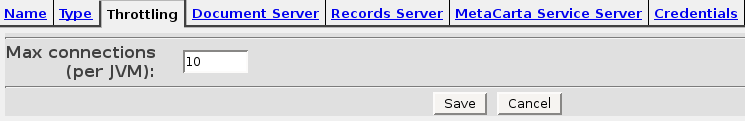
\includegraphics[width=300pt]{mer-edit-auth-tab3}

\begin{itemize}

\item \textbf{Max Connections (per JVM):} The maximum number of
connections per JVM is important for two reasons.
\ifCombinedConnectorGuide \label{max-auth}\fi First, the number of
connections may impact the resources available on your Meridio
server. You should consult your Meridio administrator about an
appropriate maximum number of connections that the crawler may use.

Second, the number of connections may impact the resources available
on the appliance. If the connector framework is slowing down your
appliance, lowering this number should help.

\end{itemize}

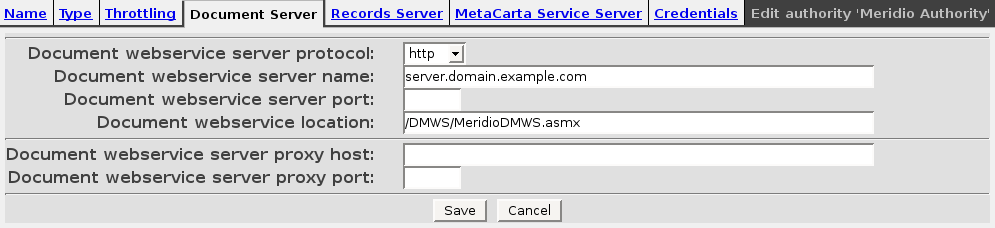
\includegraphics[width=300pt]{mer-edit-auth-tab4}

This tab specifies information about the Meridio document service that
you wish to crawl. You may need to ask your Meridio administrator for
this information.

\begin{itemize}

\item \textbf{Document webservice server protocol:} The appropriate protocol used by your Meridio document webservice, either \texttt{http://} or \texttt{https://}.

\item \textbf{Document webservice server name:} The name of the server hosting your Meridio document webservice.

\item \textbf{Document webservice server port:} The port used to connect to the Meridio document webservice.

\item \textbf{Document webservice location:} The location of the Meridio document webservice on the server specified above. By default, the location of the service is given as \dirpath{/DMWS/MeridioDMWS.asmx}.

\item \textbf{Document webservice server proxy host:} If your MetaCarta appliance must connect to the server hosting the Meridio document webservice using a proxy, specify the name of the appropriate proxy host here.

\item \textbf{Document webservice server proxy port:} The port used to connect to the proxy host.

\end{itemize}

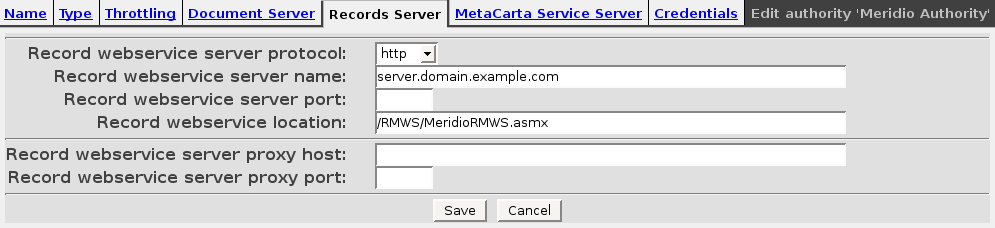
\includegraphics[width=300pt]{mer-edit-auth-tab5}


This tab specifies information about the Meridio record service
corresponding to the document service that you wish to crawl. You may
need to ask your Meridio administrator for this information. Some of
this information may be the same as from the previous tab, as a server
may host more than one Meridio service.


\begin{itemize}

\item \textbf{Record webservice server protocol:} The appropriate protocol used by your Meridio record webservice.

\item \textbf{Record webservice server name:}  The name of the server hosting your Meridio record webservice.

\item \textbf{Record webservice server port:} The port used to connect to the Meridio record webservice.

\item \textbf{Record webservice location:} The location of the Meridio record webservice on the server specified above. By default, the location of the service is given as \dirpath{/RMWS/MeridioRMWS.asmx}

\item \textbf{Record webservice server proxy host:} If your MetaCarta appliance must connect to the server hosting the Meridio record webservice using a proxy, specify the name of the appropriate proxy host here.

\item \textbf{Record webservice server proxy port:} The port used to connect to the proxy host.

\end{itemize}


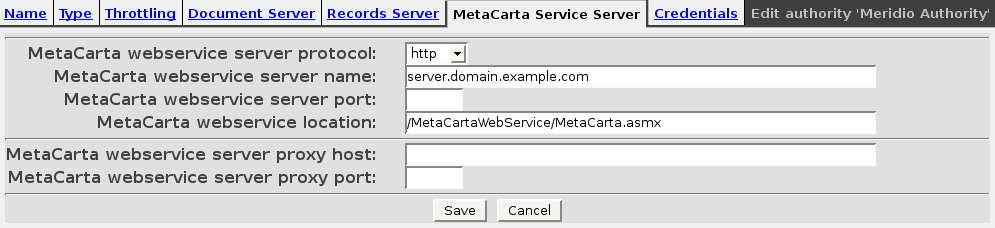
\includegraphics[width=300pt]{mer-edit-auth-tab6}


This tab specifies information about the MetaCarta Meridio Web
Service. See the Installation section, starting on page
\pageref{SWService} for a description of the service and its installation.
The server and service location will be those specified during the
installation of the service. You may need to ask your Meridio
administrator for this information.  Some of this information may be
the same as from the previous tab, as a server may host more than one
Meridio service.


\begin{itemize}

\item \textbf{MetaCarta webservice server protocol:}  The appropriate protocol used by your MetaCarta Meridio Web Service.

\item \textbf{MetaCarta webservice server name:}  The name of the server hosting your MetaCarta Meridio Web Service.

\item \textbf{MetaCarta webservice server port:}  The port used to connect to the MetaCarta Meridio Web Service.

\item \textbf{MetaCarta webservice location:}  The location of MetaCarta Meridio Web Service the on the server specified above. By default, the location of the service is given as \dirpath{/MetaCartaWebService/MetaCarta.asmx}

\item \textbf{MetaCarta webservice server proxy host:}  If your MetaCarta appliance must connect to the server hosting the MetaCarta Meridio Web Service using a proxy, specify the name of the appropriate proxy host here.

\item \textbf{MetaCarta webservice server proxy port:}  The port used to connect to the proxy host.

\end{itemize}



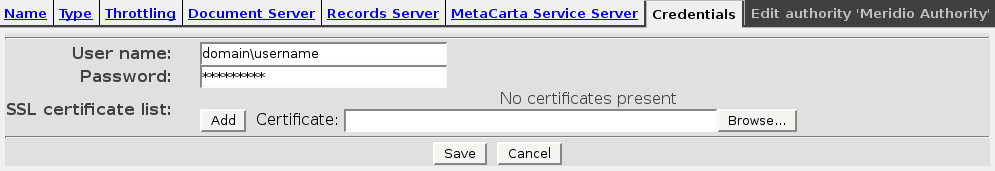
\includegraphics[width=300pt]{mer-edit-auth-tab7}

\begin{itemize}

\item \textbf{User name:} The Active Directory user name that the
appliance should use when connecting to the Meridio services, in the
form \texttt{domain$\backslash{}$username}. This should be an account
created specifically for the appliance.

% Might it be worth a pointer to instructions for doing so?
% Or at least "contact your AD administrator" if that's the right thing?

\item \textbf{Password:} The password for that account.

\item \textbf{SSL certificate list:}
You can upload SSL certificates to use with this connection here. If
you specified ``https'' as the server protocol above, you may need to
upload appropriate certificates or certificate authorities here. The
repository connection will need certificates similar to those used to
connect to your Meridio web service using an Internet browser.


If the certificate authority used to sign your server certificate is a
well-known authority, you will not need to upload a certificate
here. The appliance will automatically accept a certificate from the
server. If the server certificate is signed by an unknown authority,
you should upload the authority's certificate. In some cases, the
authority may be unavailable. In this case, you can upload the
server-side certificate itself. Server-side certificate changes may
require you to upload newer versions of this certificate if you use
this option.


\end{itemize}


After entering this information, you will be taken to the authority
connection status page for this authority:

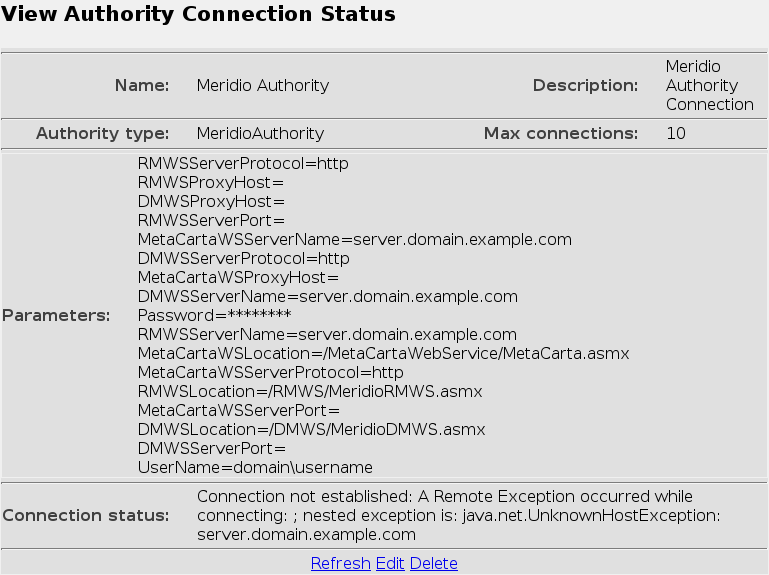
\includegraphics[width=300pt]{mer-view-auth-conn-status}

In this example (which does not contain accurate information for any
Meridio server), the Connection Status is ``Connection not established.''
If you see this message, you may have entered incorrect data into one
of the fields, and should click ``Edit'' to fix the data. If you have
entered everything as you intended, please inform your Meridio
administrator; you may not have been given the correct information,
or one of the services might be down.

